\subsection[\texorpdfstring{$\textup{N}^3\textup{LO}$ in the HTL}{N3LO in the HTL}]{\texorpdfstring{\boldmath$\textup{N}^3\textup{LO}$ in the HTL}{N3LO in the HTL}}

%\textit{Authors:} Long-Bin Chen, Hai Tao Li, Hua-Sheng Shao, Jian Wang (1909.06808)

\textbf{Long-Bin Chen, Xuan Chen, Yuesheng Dai, Hai Tao Li, Shi-Yuan Li, Hua-Sheng Shao, Jian Wang~\cite{Chen:2019lzz,Chen:2026zmi}.}



\begin{figure}[!hbtp]
    \centering
    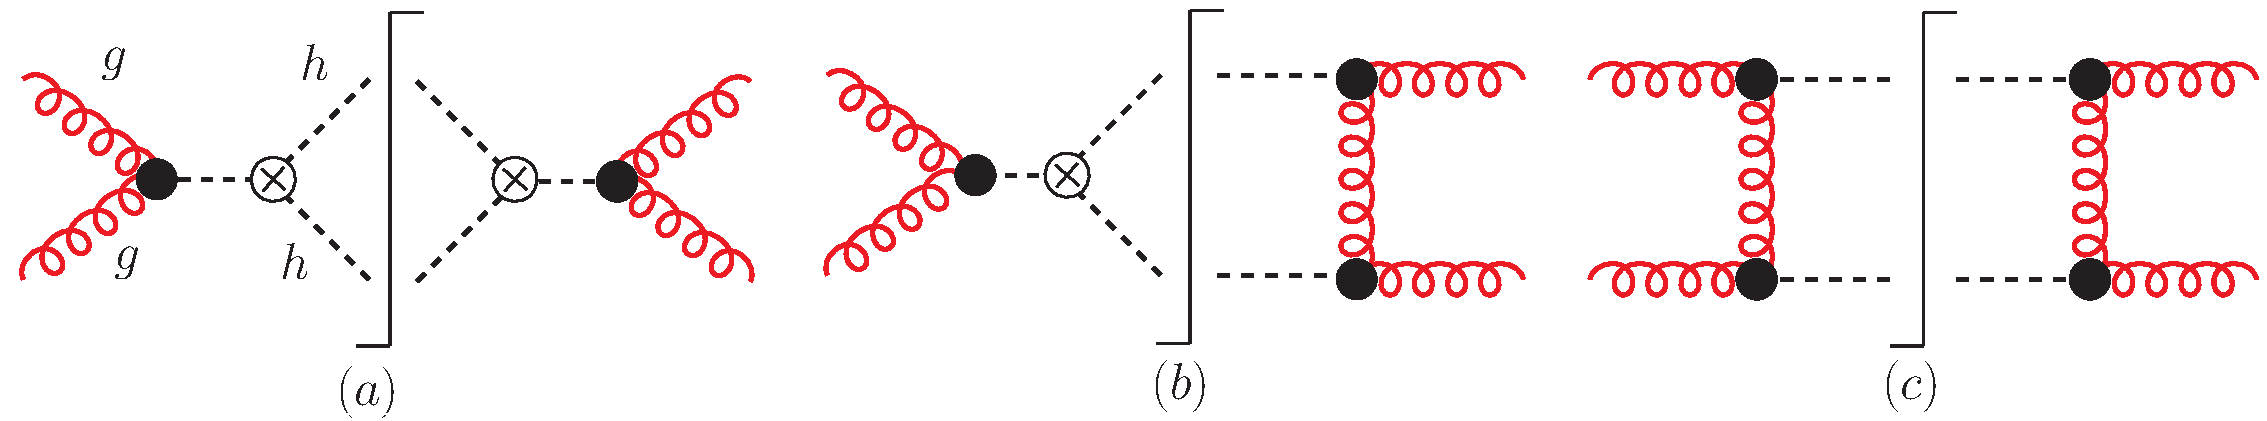
\includegraphics[width=\textwidth]{N3LO_QCD_SM/N3LO_htl/Images/feyn_HH}
    \caption{Representative Born-level cut diagrams for Higgs boson pair production via gluon-gluon fusion. Bullets denote the effective vertices described by the Lagrangian in Eq.~\eqref{eq:effL}, while the crossed circle represents the trilinear Higgs boson self-coupling. Figure adapted from Ref.~\cite{Chen:2019lzz}.}
    \label{fig:FeynDia}
\end{figure}

\noindent The fixed-order computation of the gluon-gluon fusion (ggF) Higgs boson pair cross section in the HTL can be organized according to the number of the effective-vertex insertions in the squared amplitude. Three representative Born-level cut diagrams are shown in Fig.~\ref{fig:FeynDia}: from left to right, they involve two, three, and four effective vertices, and are denoted as class-$a$, class-$b$, and class-$c$ contributions, respectively. Accordingly, the phase-space-integrated or differential cross section can be decomposed as
\begin{align}
    d\sigma_{hh} = d\sigma^{a}_{hh} + d\sigma^{b}_{hh} + d\sigma^{c}_{hh} .
\end{align}
Their contributions at different powers of $\alpha_s$ are summarized in Table~\ref{tab:my_label}. To achieve N$^3$LO accuracy in $\alpha_s$, the required inputs are the class-$a$ contribution at $\mathrm{N^3LO}_a$, the class-$b$ contribution at $\mathrm{NNLO}_b$, and the class-$c$ contribution at $\mathrm{NLO}_c$, where the subscripts indicate the perturbative order within the corresponding topology class.

\begin{table}[hbt!]
    \centering
%    \begin{tabular}{c|c|c|c|c}
%    \begin{tabular}{ccccc}
%%    \hline \hline
%    \toprule
%        &  LO  & NLO  & NNLO  & $\textup{N}^3\textup{LO}$  \\
%%    \hline
%    \midrule
%    Class  &  $\mathcal{O}(\alpha_s^2)$  &   $\mathcal{O}(\alpha_s^3)$ &   $\mathcal{O}(\alpha_s^4)$  & $\mathcal{O}(\alpha_s^5)$
%     \\
%%    \hline
%    \midrule
%    \multirow{2}{*}{$a$}
%     &  $\textup{LO}_a$  &   $\textup{NLO}_a$ &   $\textup{NNLO}_a$  & $\textup{N}^3\textup{LO}_a$
%     \\
%      &  $\mathcal{O}(\alpha_s^2)$  &   $\mathcal{O}(\alpha_s^3)$ &   $\mathcal{O}(\alpha_s^4)$  & $\mathcal{O}(\alpha_s^5)$
%     \\
%%    \hline
%    \midrule
%     \multirow{2}{*}{$b$}
%     &  --- &   $\textup{LO}_b$ &   $\textup{NLO}_b$  &  $\textup{NNLO}_b$
%     \\
%     &  0 &   $\mathcal{O}(\alpha_s^3)$ &   $\mathcal{O}(\alpha_s^4)$  & $\mathcal{O}(\alpha_s^5)$
%     \\
%%    \hline
%    \midrule
%    \multirow{2}{*}{$c$}
%      & --- &  --- &   $\textup{LO}_c$  & $\textup{NLO}_c$
%     \\
%       & 0 &  0 &   $\mathcal{O}(\alpha_s^4)$  & $\mathcal{O}(\alpha_s^5)$
%     \\
%%     \hline \hline
%    \bottomrule
%    \end{tabular}
\begin{tabular}{ccccc}
    \toprule
        \multirow{2}{*}{Class}    &  LO  & NLO  & NNLO  & $\textup{N}^3\textup{LO}$  \\
      &  $\mathcal{O}(\alpha_s^2)$  &   $\mathcal{O}(\alpha_s^3)$ &   $\mathcal{O}(\alpha_s^4)$  & $\mathcal{O}(\alpha_s^5)$
     \\
    \midrule
    $a$ &  $\textup{LO}_a$  &   $\textup{NLO}_a$ &   $\textup{NNLO}_a$  & $\textup{N}^3\textup{LO}_a$
     \\
     $b$ &  --- &   $\textup{LO}_b$ &   $\textup{NLO}_b$  &  $\textup{NNLO}_b$
     \\
    $c$ & --- &  --- &   $\textup{LO}_c$  & $\textup{NLO}_c$
     \\
    \bottomrule
    \end{tabular}
            \caption{Perturbative orders in $\alpha_s$ for three topology classes.
    The first and second rows indicate the perturbative expansion orders of the total cross section for Higgs boson pair production,
    while each individual class has its own expansion order, specified by the subscript.}
    \label{tab:my_label}
\end{table}

The class-$a$ contribution can be obtained from the single-Higgs production cross section in the HTL up to N$^3$LO.
For inclusive results, this component is computed using the public program \texttt{iHixs2}~\cite{Dulat:2018rbf}, while the class-$a$ contribution for fully differential results is computed with \texttt{NNLOJet}~\cite{NNLOJET:2025rno} using the $q_T$ phase-space slicing ($q_T$-slicing) method~\cite{Catani:2007vq,Cieri:2018oms}.
The class-$b$ contribution is calculated up to NNLO in $\alpha_s$ using the $q_T$-slicing method~\cite{Catani:2007vq} by combining the \texttt{MadGraph5\_aMC@NLO}~\cite{Alwall:2014hca,Frederix:2018nkq} framework with a private code. The corresponding two-loop amplitude with two effective-vertex insertions was computed in Ref.~\cite{Banerjee:2018lfq}. The double-real and real-virtual contributions in class-$b$, as well as all contributions in class-$c$, are calculated using \texttt{MadGraph5\_aMC@NLO}.

\begin{table}[h]
\begin{center}

\newcolumntype{P}[1]{>{\centering\arraybackslash}p{#1}}
{\renewcommand{\arraystretch}{1.5}
%\begin{tabular}{|P{2.7cm}|P{2.7cm}|P{2.7cm}|P{2.7cm}|}
\begin{tabular}{P{2.7cm}P{2.7cm}P{2.7cm}P{2.7cm}}
\toprule
    & $\sigma_{{\rm NLO}}$ $[\textup{fb}]$
    & $\sigma_{{\rm NNLO}}$ $[\textup{fb}]$
    & $\sigma_{{\rm N}^3{\rm LO}}$ $[\textup{fb}]$
    \\
  \midrule
  Inclusive &
  $31.89^{+18\%}_{-15\%}$ &
  $37.55^{+5.2\%}_{-7.6\%}$ &
 $38.65^{+0.5\%}_{-2.7\%}$
 \\
 \midrule
   Fiducial &
  $27.87_{-15 \%}^{+18 \%}$ &
  $32.74_{-7.3 \%}^{+5.2 \%}$ &
 $34.00(4)_{-2.9 \%}^{+1.4 \%}$
 \\
 \bottomrule
\end{tabular}}
\caption{Fixed-order cross sections in the HTL at $\sqrt{s}=14\,\textup{TeV}$. The second line corresponds to the inclusive case, while the third line corresponds to the fiducial case with cuts defined in Eq.~\eqref{eq:fiducialcuts}. The quoted uncertainties are obtained from $7$-point scale variations.}
\label{tab:FON3LOinclusivexs}
%\end{small}
\end{center}
\end{table}

\begin{figure*}[t]
\centering
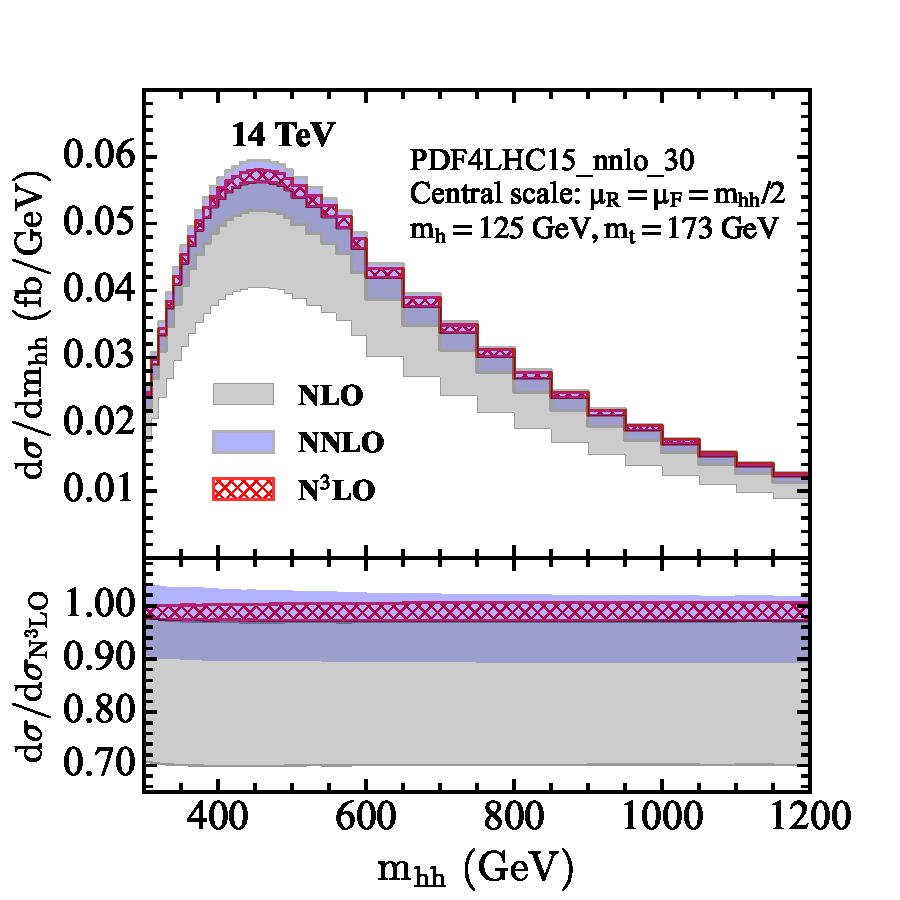
\includegraphics[width=0.49\textwidth]{N3LO_QCD_SM/N3LO_htl/Images/diff_large_mt_13_14_FO_CERNYR5}
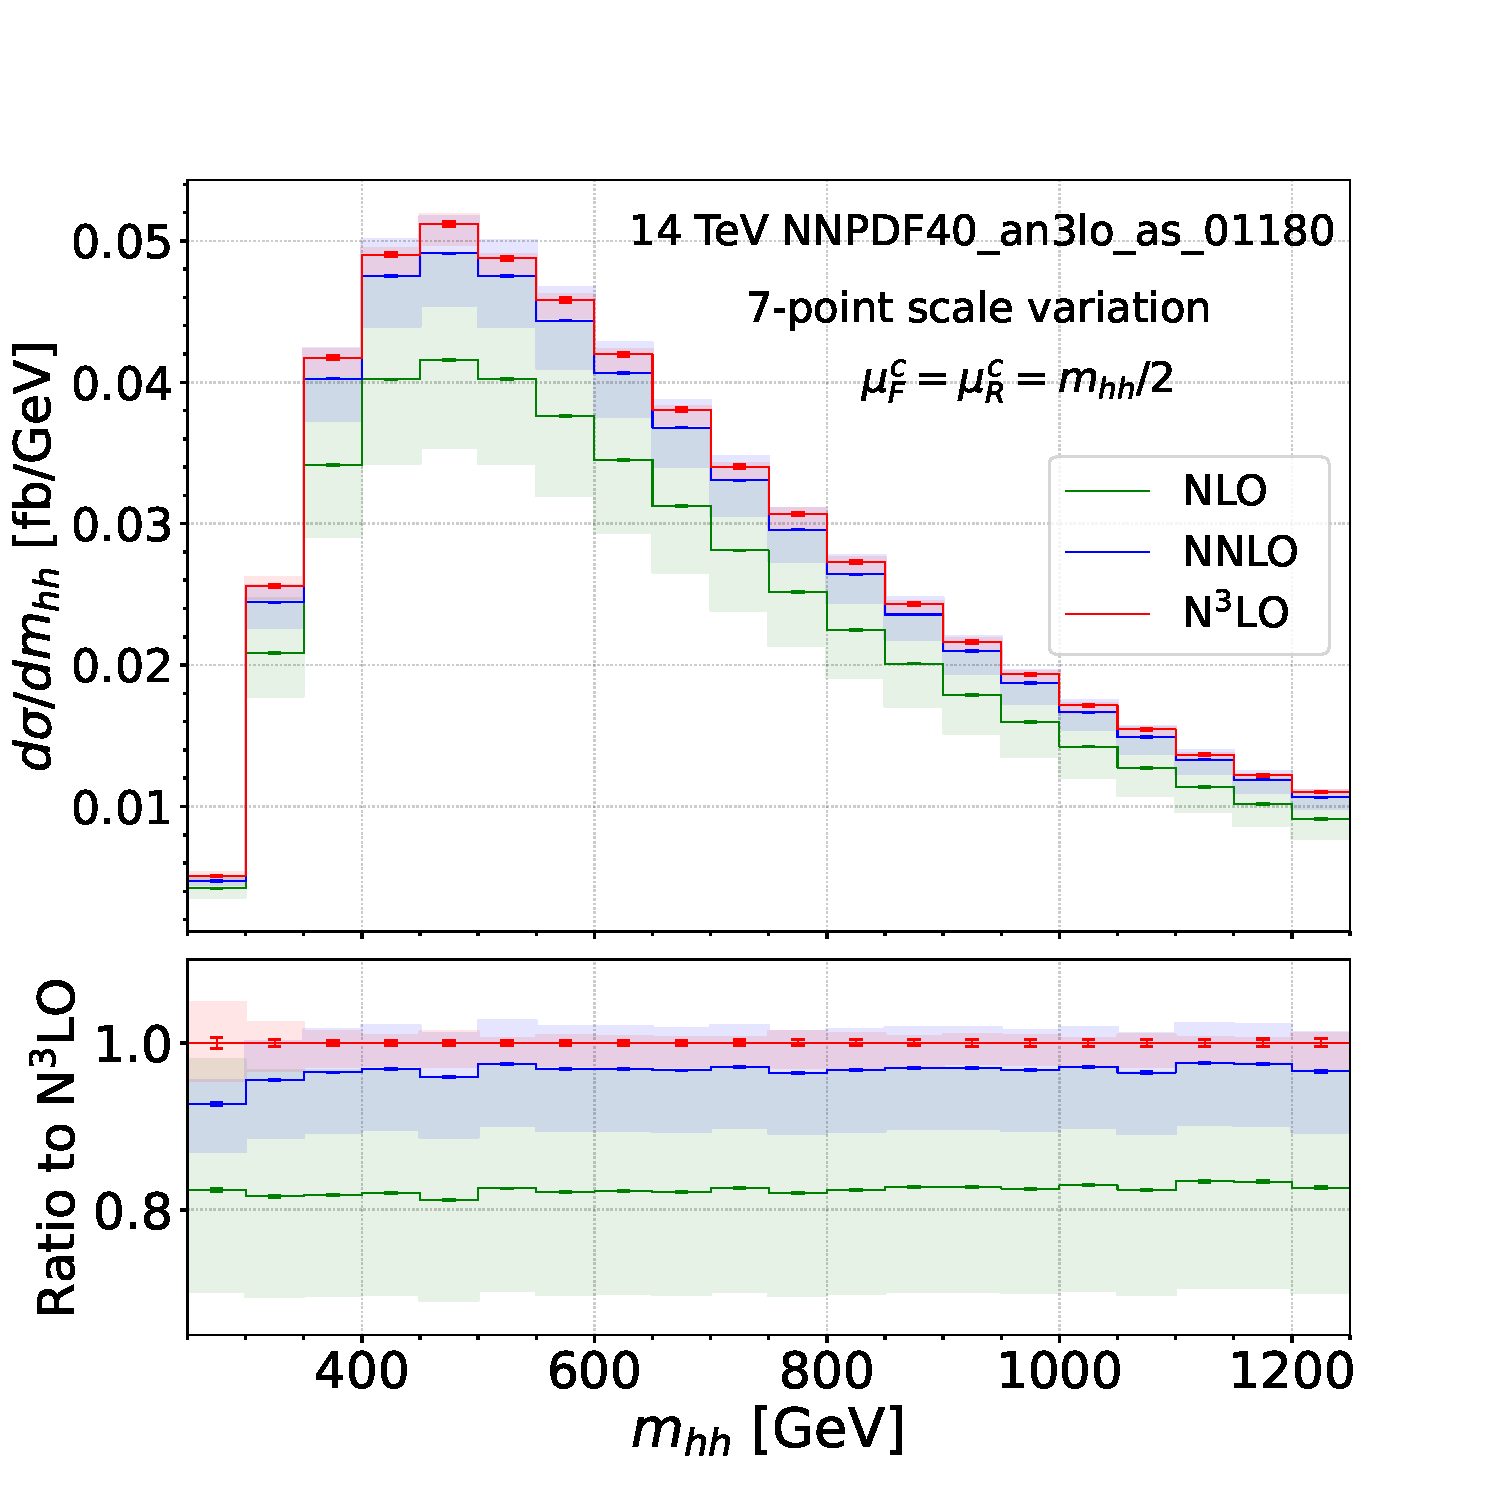
\includegraphics[width=0.49\textwidth,height=7.52cm]{N3LO_QCD_SM/N3LO_htl/Images/HH_m_hh}
\caption{Inclusive (left) and fiducial (right) invariant-mass distributions for Higgs boson pair production at $\sqrt{s}=14$ TeV in the HTL, from NLO to N$^3$LO. The error bands correspond to $7$-point scale variations. Here $\mu^C$ denotes the central value of the renormalization and factorization scales. Results shown are from Refs.~\cite{Chen:2019lzz,Chen:2019fhs,Chen:2026zmi}.}
\label{fig:xs_vs_mhh_FO_N3LO}
\end{figure*}


\begin{figure*}[ht]
\centering
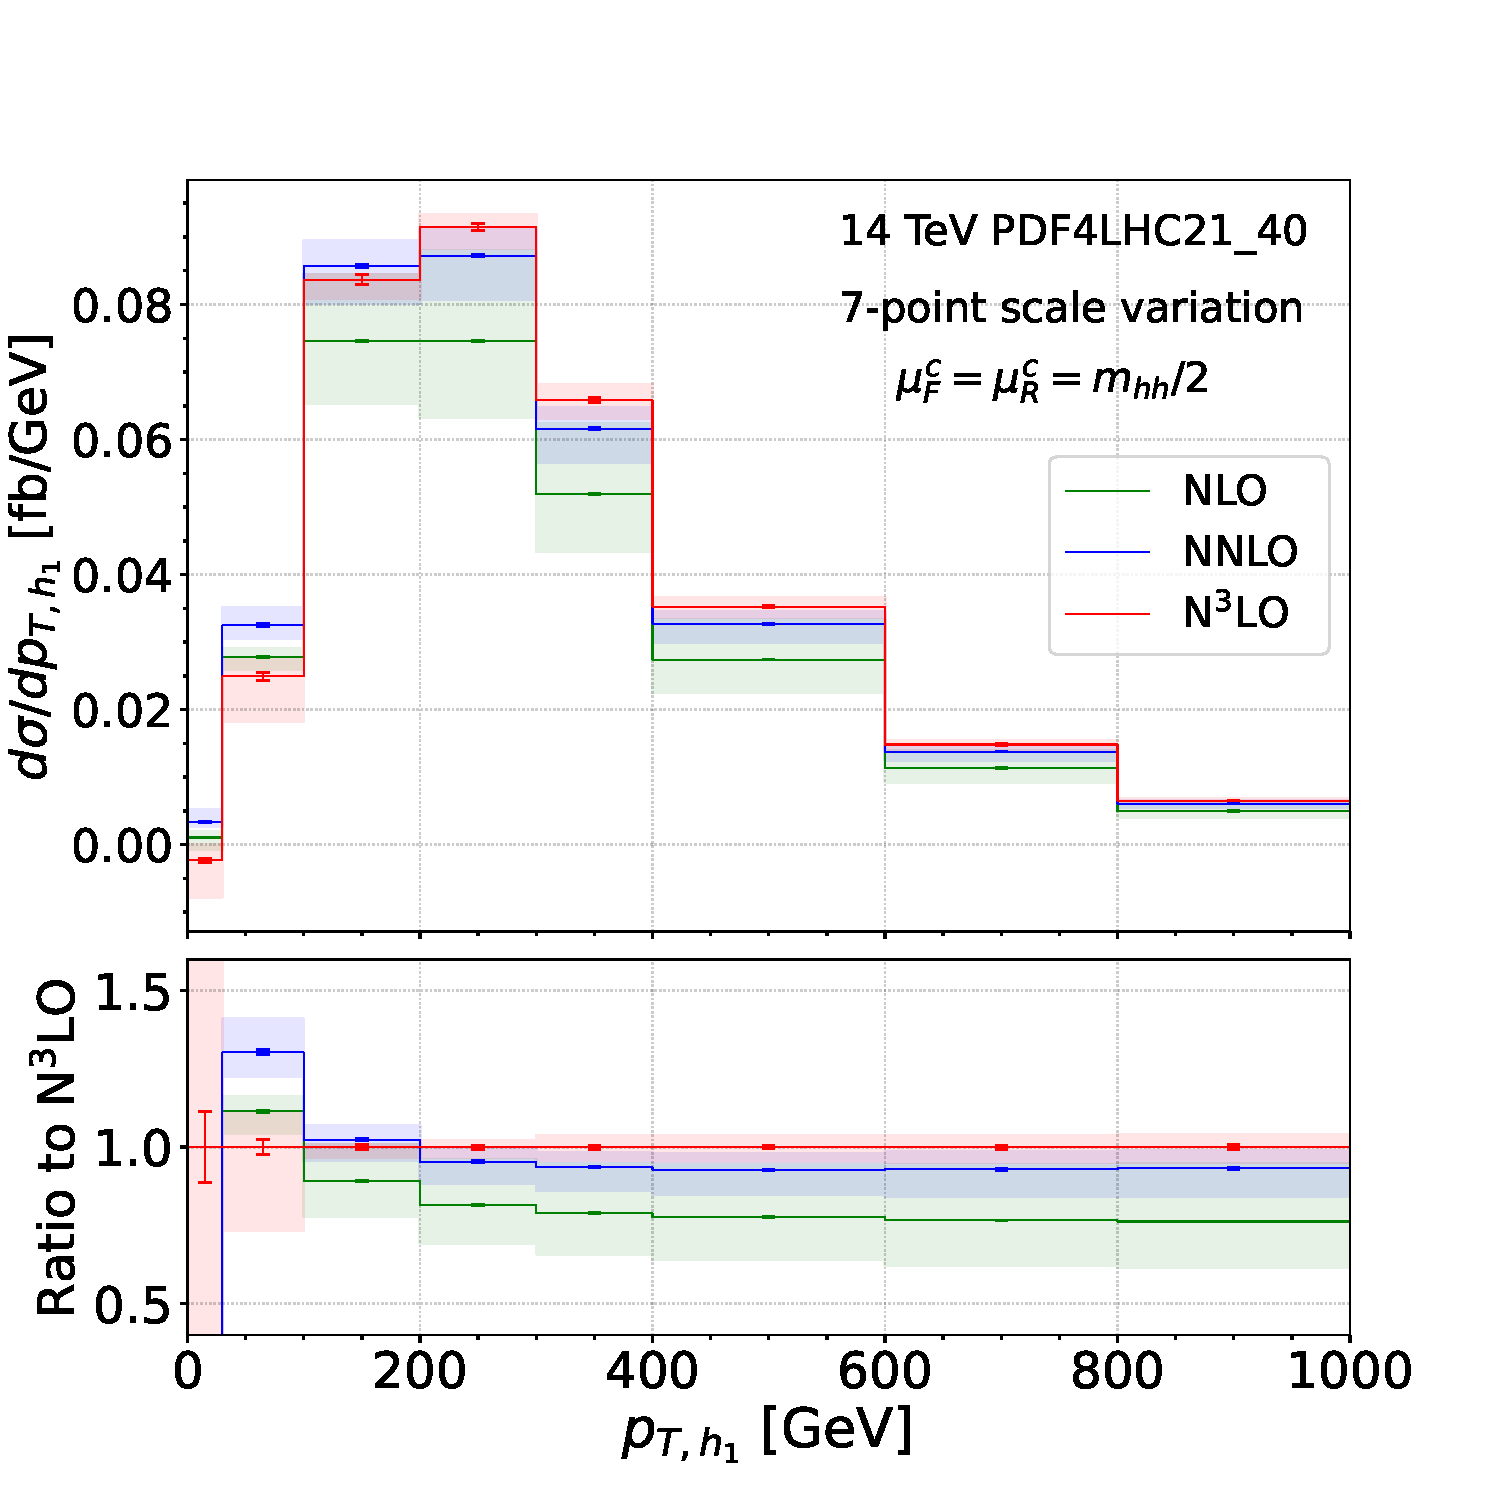
\includegraphics[width=0.49\textwidth,height=7.52cm]{N3LO_QCD_SM/N3LO_htl/Images/HH_pt_h1st_100.pdf}
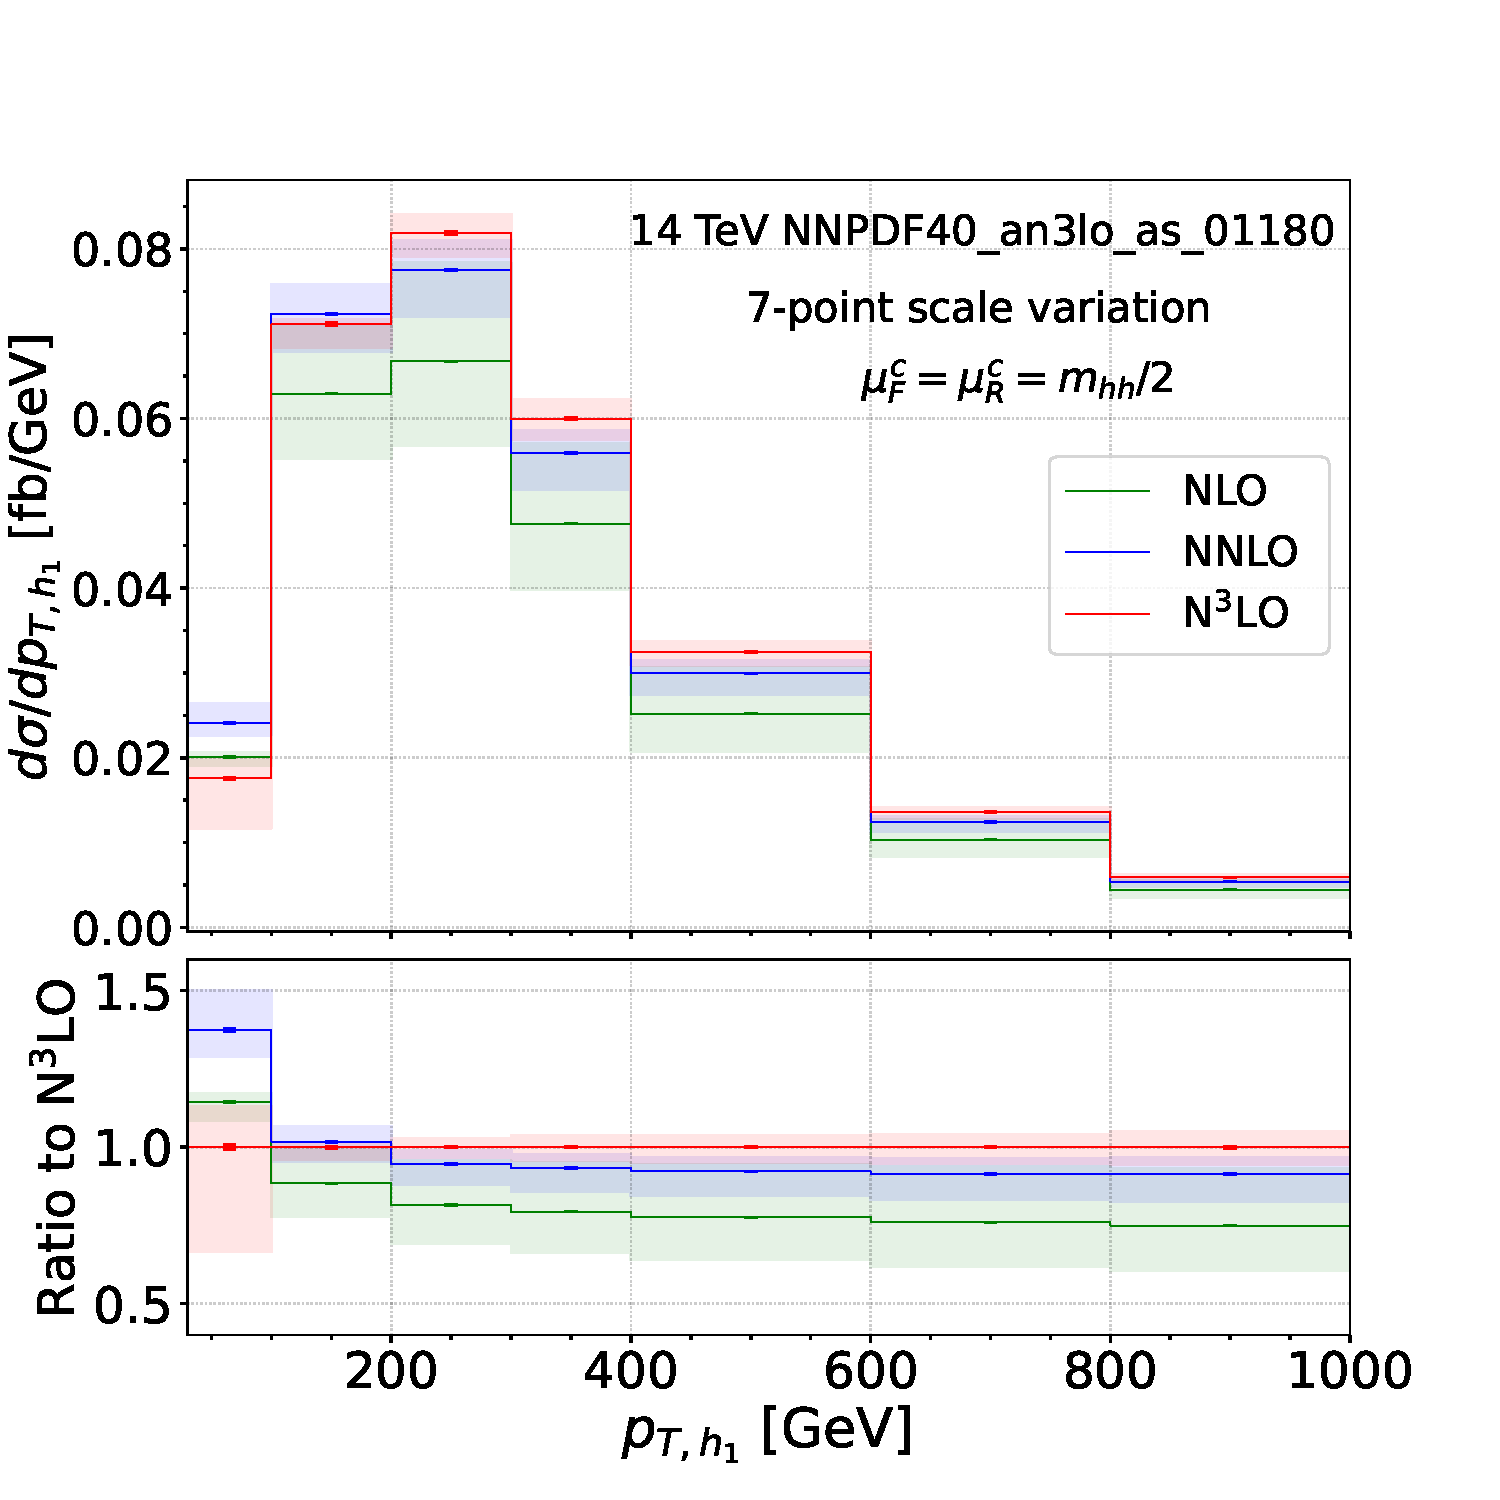
\includegraphics[width=0.49\textwidth,height=7.52cm]{N3LO_QCD_SM/N3LO_htl/Images/HH_pt_h1st.pdf}
\caption{Inclusive (left) and fiducial (right) leading-Higgs $p_{T}$ distributions for Higgs boson pair production at $\sqrt{s}=14$ TeV in the HTL, from NLO to N$^3$LO. The error bands correspond to $7$-point scale variations. Here $\mu^C$ denotes the central value of the renormalization and factorization scales. Results shown are from Ref.~\cite{Chen:2026zmi}.}
\label{fig:fid_pth1_FO_N3LO}
\end{figure*}


\begin{figure*}[ht]
\centering
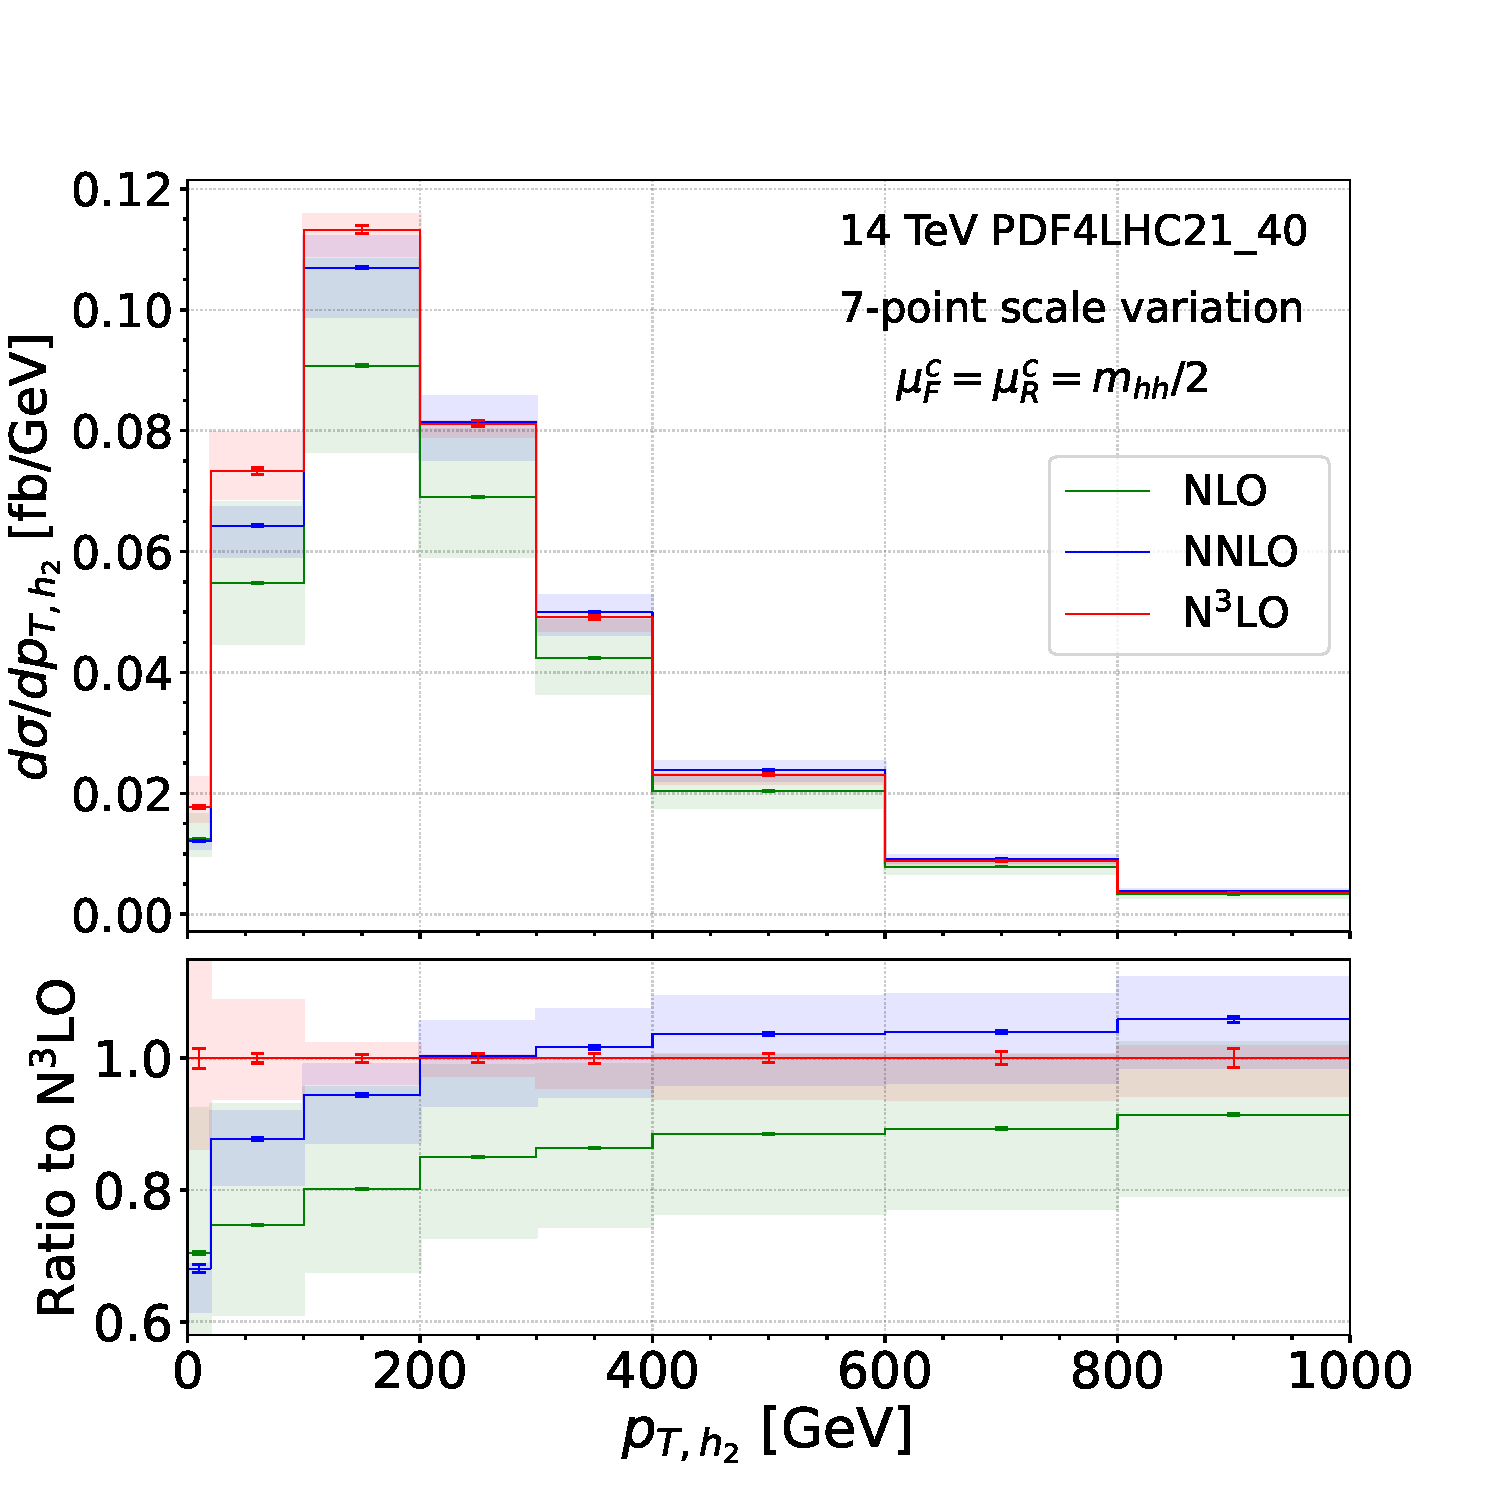
\includegraphics[width=0.49\textwidth,height=7.52cm]{N3LO_QCD_SM/N3LO_htl/Images/HH_pt_h2nd_100.pdf}
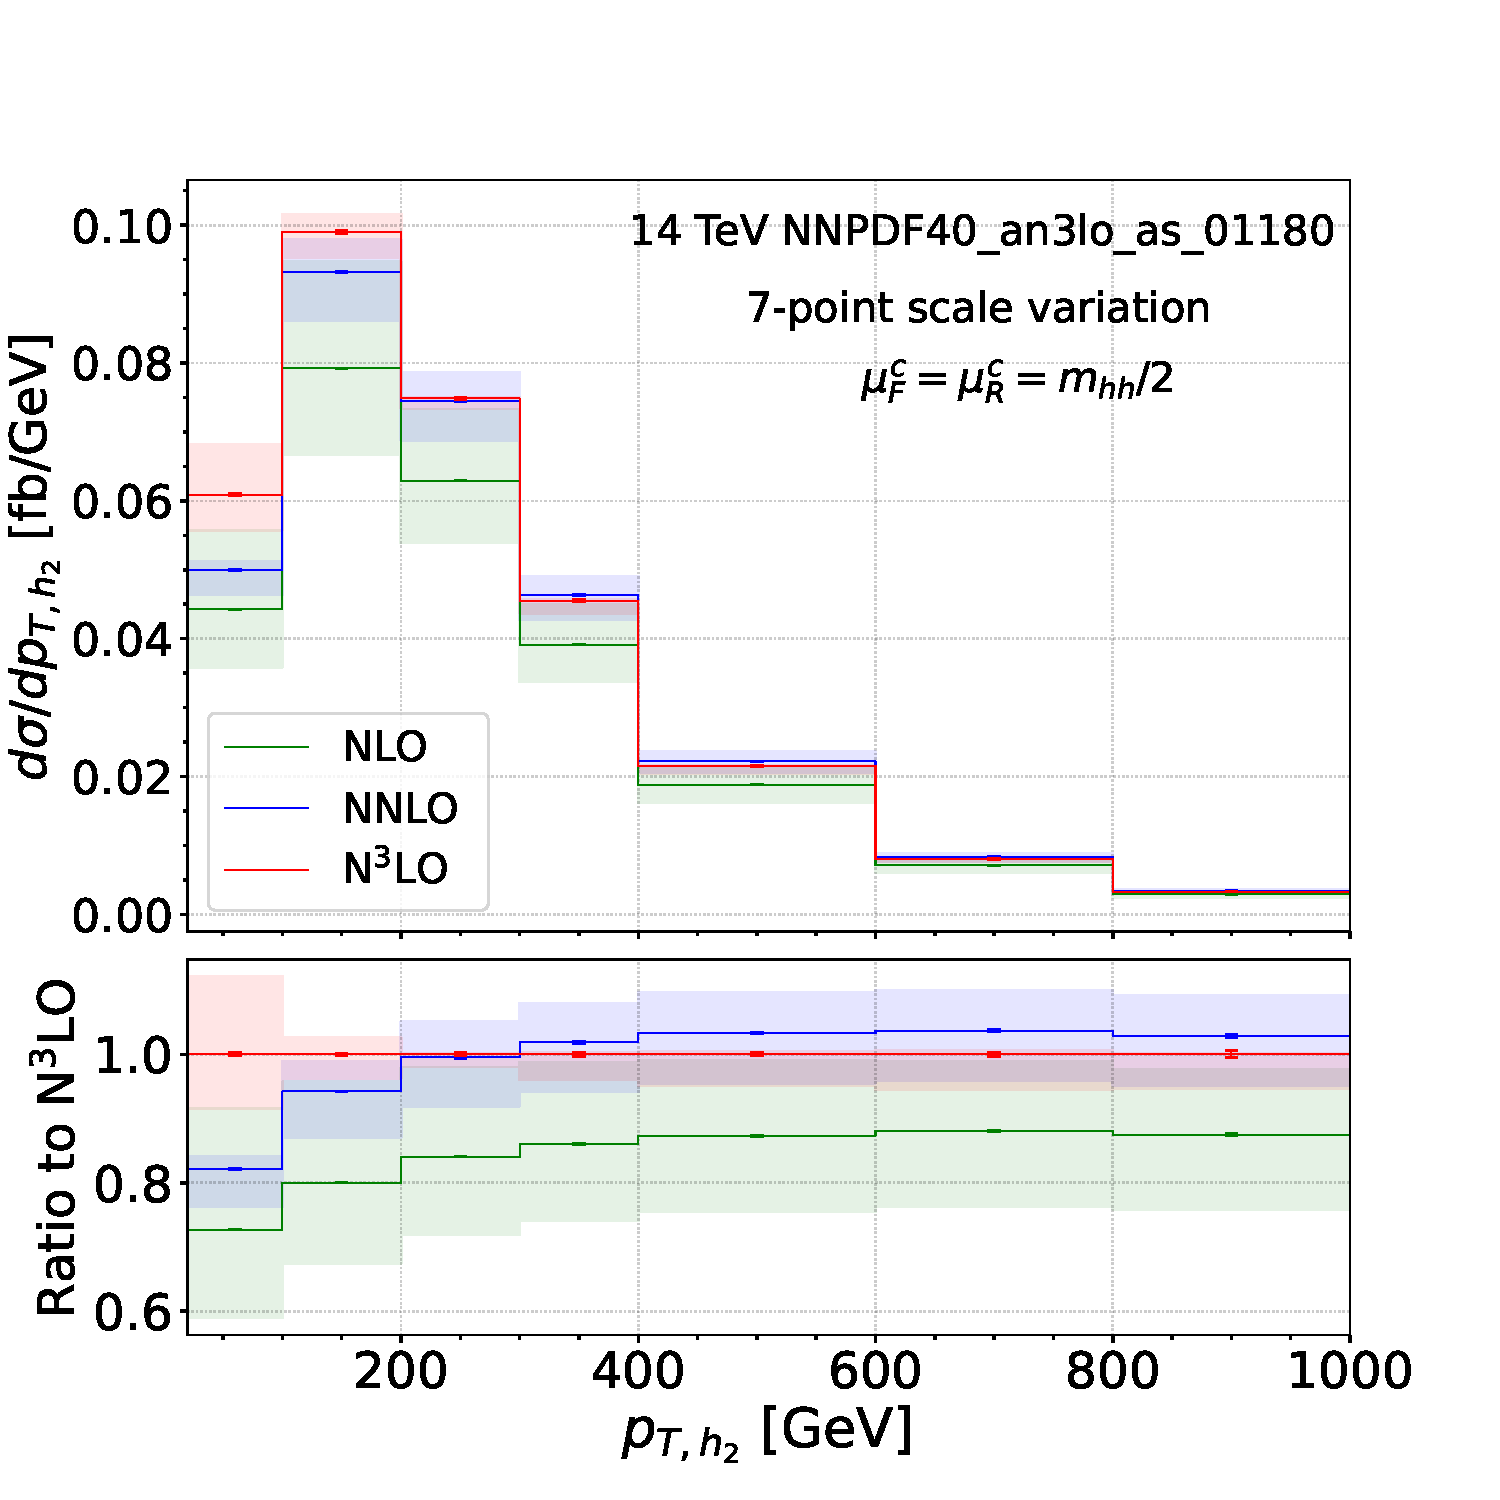
\includegraphics[width=0.49\textwidth,height=7.52cm]{N3LO_QCD_SM/N3LO_htl/Images/HH_pt_h2nd.pdf}
\caption{Inclusive (left) and fiducial (right) subleading-Higgs $p_{T}$ distributions for Higgs boson pair production at $\sqrt{s}=14$ TeV in the HTL, from NLO to N$^3$LO. The error bands correspond to $7$-point scale variations. Here $\mu^C$ denotes the central value of the renormalization and factorization scales. Results shown are from Ref.~\cite{Chen:2026zmi}.
}
\label{fig:fid_pth2_FO_N3LO}
\end{figure*}


The phase-space-integrated cross sections from NLO to N$^3$LO in the HTL at $\sqrt{s}=14$ TeV for proton-proton ($pp$) collisions are listed in Table~\ref{tab:FON3LOinclusivexs}. For the inclusive (fiducial) results, the N$^3$LO QCD corrections increase the NNLO cross section by $3\%$ ($4\%$) and reduce the fractional scale uncertainty by a factor of four (three).
The Higgs boson pair invariant-mass distributions at fixed orders in $\alpha_s$ are shown in Fig.~\ref{fig:xs_vs_mhh_FO_N3LO} for the inclusive (left panel) and fiducial (right panel) cases. In both cases, the higher-order QCD corrections do not shift the peak positions of the distributions. There is, however, a small difference between the two setups. In the inclusive case, the $K$-factor for N$^3$LO over NNLO is nearly flat across a wide range of $m_{hh}$, and the N$^3$LO prediction, with its small scale uncertainty, lies entirely within the NNLO uncertainty band. In contrast, with the fiducial cuts defined in Eq.~\eqref{eq:fiducialcuts}, the N$^3$LO correction in the first bin ($m_{hh}<300$ GeV) amounts to 8$\%$, which is almost a factor of two larger than the corrections in the other bins. Additionally, the scale uncertainty is significantly larger in this bin. The difference in the threshold region mainly stems from linear power corrections in the presence of fiducial cuts. The leading- and subleading-$p_T$ distributions of the two Higgs bosons are shown in Figs.~\ref{fig:fid_pth1_FO_N3LO} and~\ref{fig:fid_pth2_FO_N3LO}. The N$^3$LO QCD corrections modify their shapes, with the largest effects occurring in the small-$p_T$ region, where the scale uncertainties are also most significant. In this region, the fixed-order predictions are not stable, and a resummation calculation is necessary to stabilize the theoretical predictions. Moreover, the fiducial cuts also have a clear impact in this region. The scale uncertainty at N$^3$LO of $p_{T,h_1}$ ($p_{T,h_2}$) in the 20--100 GeV (30--100 GeV) bin changes from 38$\%$ (15$\%$) to 46$\%$ (21$\%$) after imposing the fiducial cuts.
In the intermediate- and large-$p_T$ regions, the fixed-order predictions remain reliable.
